% Figure from MATH 591 notes, section 3. Compile with the notes preamble.
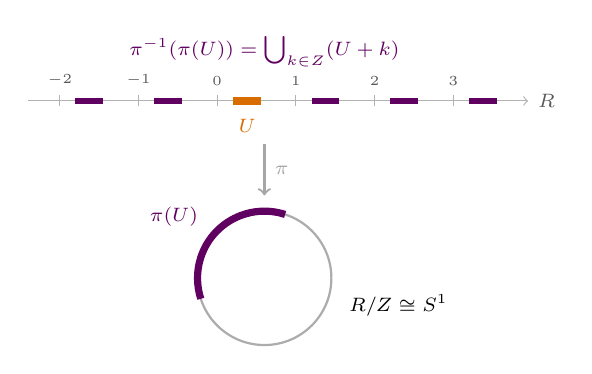
\begin{tikzpicture}
\draw[->, gray!60] (-2.4,0) -- (3.95,0) node[right, font=\scriptsize, text=gray!70!black] {$\mathbb{R}$};
\draw[gray!60] (-2,-0.07) -- (-2,0.07) node[above, font=\tiny, text=gray!70!black] {$-2$};
\draw[gray!60] (-1,-0.07) -- (-1,0.07) node[above, font=\tiny, text=gray!70!black] {$-1$};
\draw[gray!60] (0,-0.07) -- (0,0.07) node[above, font=\tiny, text=gray!70!black] {$0$};
\draw[gray!60] (1,-0.07) -- (1,0.07) node[above, font=\tiny, text=gray!70!black] {$1$};
\draw[gray!60] (2,-0.07) -- (2,0.07) node[above, font=\tiny, text=gray!70!black] {$2$};
\draw[gray!60] (3,-0.07) -- (3,0.07) node[above, font=\tiny, text=gray!70!black] {$3$};
\draw[violet!75!black, line width=2.2pt] (-1.80,0) -- (-1.45,0);
\draw[violet!75!black, line width=2.2pt] (-0.80,0) -- (-0.45,0);
\draw[violet!75!black, line width=2.2pt] (0.20,0) -- (0.55,0);
\draw[violet!75!black, line width=2.2pt] (1.20,0) -- (1.55,0);
\draw[violet!75!black, line width=2.2pt] (2.20,0) -- (2.55,0);
\draw[violet!75!black, line width=2.2pt] (3.20,0) -- (3.55,0);
\draw[orange!85!black, line width=3.2pt] (0.20,0) -- (0.55,0); \node[orange!85!black, font=\scriptsize] at (0.38,-0.32) {$U$};
\node[violet!75!black, font=\scriptsize] at (0.6,0.62) {$\pi^{-1}(\pi(U)) = \bigcup_{k\in\mathbb{Z}} (U + k)$};
\draw[->, thick, gray!70] (0.6,-0.55) -- node[right, font=\scriptsize] {$\pi$} (0.6,-1.2);
\draw[thick, gray!65] (0.60,-2.25) circle (0.85);
\draw[violet!75!black, line width=2.6pt] (0.60,-2.25) ++(72.0:0.85) arc (72.0:198.0:0.85);
\node[violet!75!black, font=\scriptsize, anchor=south east] at (-0.12,-1.72) {$\pi(U)$};
\node[font=\scriptsize, anchor=west] at (1.55,-2.60) {$\mathbb{R}/\mathbb{Z} \cong S^1$};
\end{tikzpicture}
